\documentclass{article}
\usepackage[margin=1in]{geometry}
\usepackage{amsmath,amsthm,amssymb}
\usepackage{bbm,enumerate,mathtools}
\usepackage{tikz,pgfplots}
\usepackage{chessboard}
\usepackage[hidelinks]{hyperref}
\usepackage{multicol} % Problem 35

\newenvironment{question}{\begin{trivlist}\item[\textbf{Question.}]}{\end{trivlist}}
\newenvironment{note}{\begin{trivlist}\item[\textbf{Note.}]}{\end{trivlist}}
\newenvironment{references}{\begin{trivlist}\item[\textbf{References.}]}{\end{trivlist}}
\newenvironment{related}{\begin{trivlist}\item[\textbf{Related.}]\end{trivlist}\begin{enumerate}}{\end{enumerate}}


\begin{document}
\rating{3}{1}
For two positive real numbers $a > b \in \mathbb{R}_+$ consider the part of the
two spirals parameterized by \begin{align*}
  \vec{x}_a(t) &= (at\cos(2\pi t), at\sin(2\pi t)) \text{ for } t \in \left[0,\frac{b}{a-b}\right] \text{ and}\\
  \vec{x}_b(t) &= (bt\cos(2\pi t), bt\sin(2\pi t)) \text{ for } t \in \left[0,\frac{a}{a-b}\right],
\end{align*}\\[-10pt] which lie within a circle of radius $\displaystyle r=\frac{ab}{a-b}$

If we look at the area between the curves, we can see that the area between
the curves is precisely \(\frac{1}{3}\pi r^2\).
Moreover, if we look at the area of this region that lies inside of a circle of
radius $r_*$ for $r_* \in (0, r]$, we find the area is \(
  \pi r_*^2 \left(1 - \frac23\frac{r_*}{r}\right)
\)
\begin{figure}[ht!]
  ~
  \hfill
  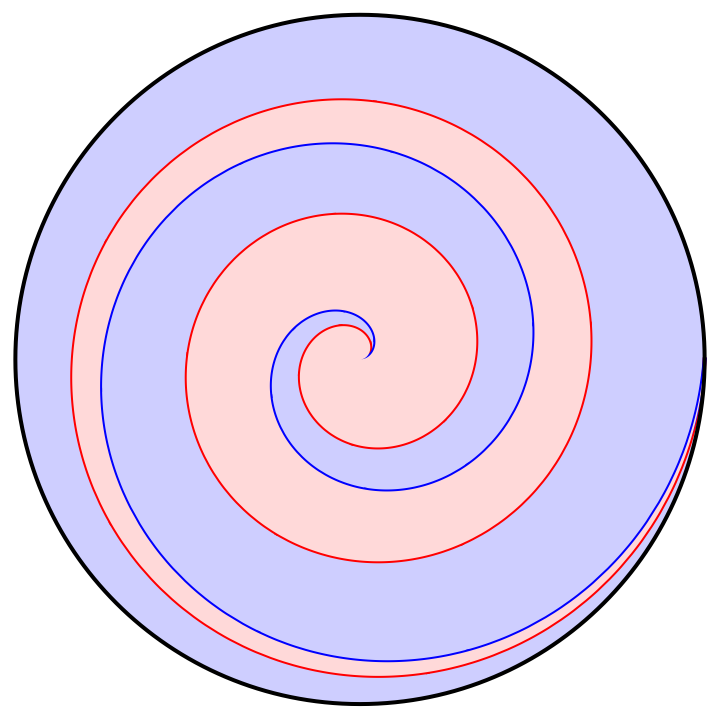
\includegraphics[width=0.3\textwidth]{assets/132_problem/spiral_100.png}
  \hfill
  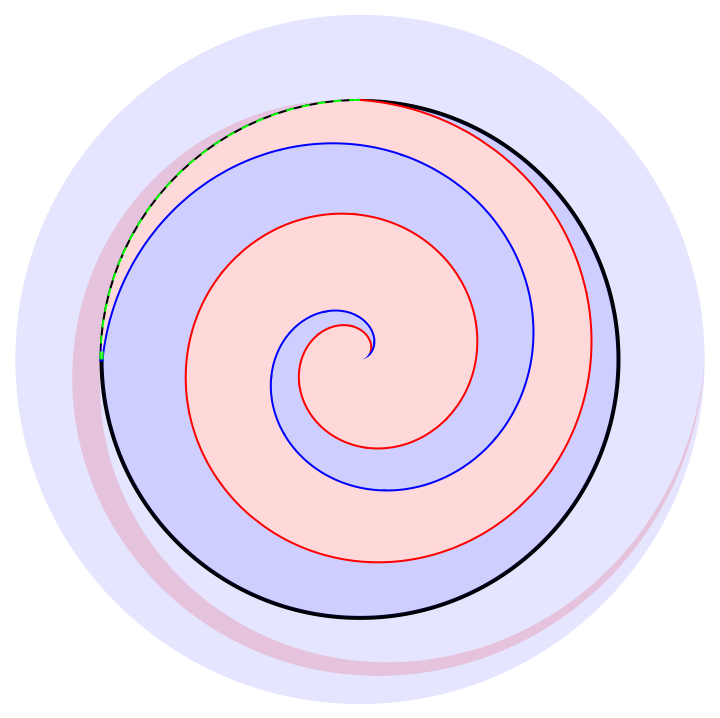
\includegraphics[width=0.3\textwidth]{assets/132_problem/spiral_075.png}
  \hfill
  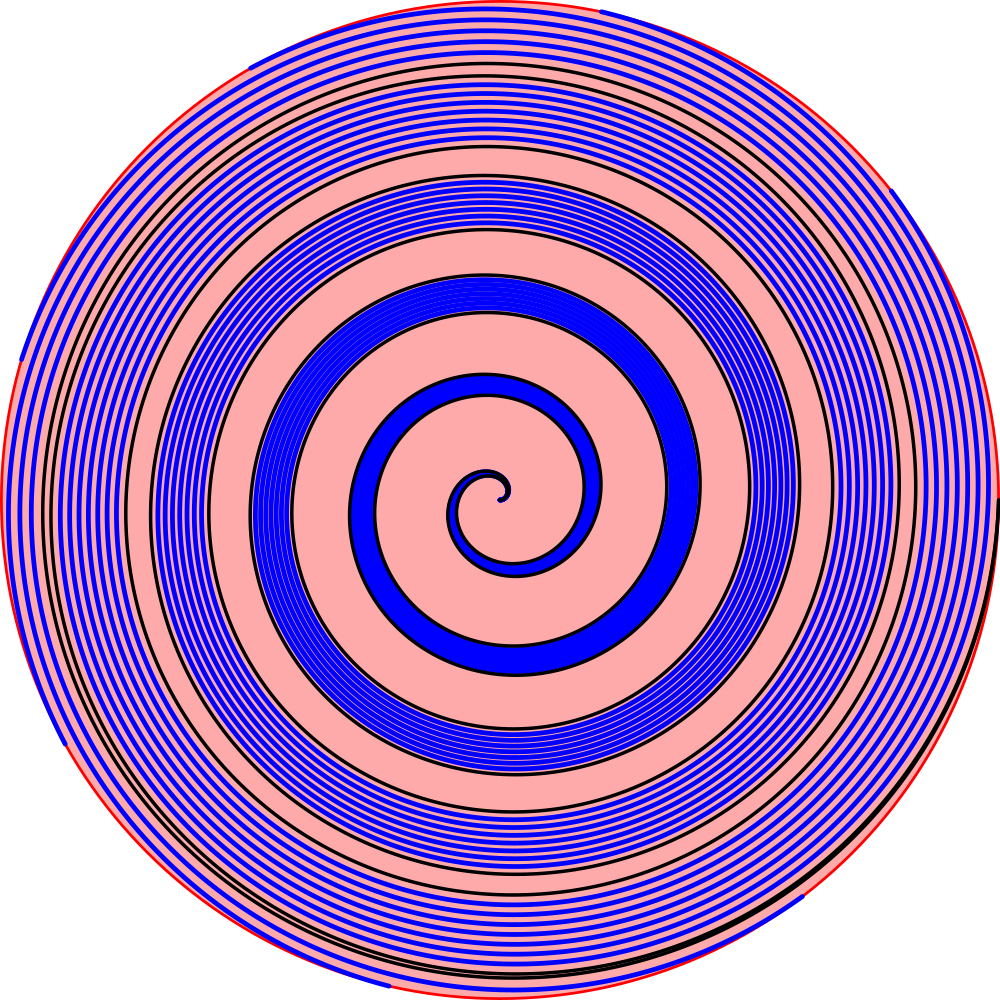
\includegraphics[width=0.3\textwidth]{assets/132_problem/outside_spiral.png}
  \caption{
    The area between the two curves is drawn in red, and is $1/3$ the area of the
    circle.
    In the second illustration the area between the two curves is drawn in red,
    and the region inside of the circle of radius $\frac34r$ is precisely half
    of that circle.
  }
\end{figure}

\begin{question}
  Is there an elementary proof of this?
\end{question}

\begin{related}
  \item Is there a natural way to extend $r^* > r$?
  \item Are there analogous results if $\vec{c}_f = f(t)\left(\cos(2\pi t), \cos(2\pi t)\right)$
  for some well-behaved pair of functions $f_1$ and $f_2$?
  \item Are there analogous ways to chop up the (hyper)sphere?
\end{related}

\begin{references}
  \item \href{https://web.calstatela.edu/faculty/hmendel/Ancient%20Mathematics/Pappus/Bookiv/Pappus.iv.21-25/Pappus.iv.21_25.html#Prop.%2023}{Pappus on Archimedes' spiral translated by Henry Mendell, Cal State LA}.
\end{references}
\begin{note}
  We can prove this in two ways with multivariable calculus: \begin{enumerate}
    \item Green's theorem to set up an vector line integral over the
    boundary of the region where the vector field is
    \(\vec{F}(x, y) = (-y/2, x/2)\), and
    \item Parameterizing the points in the complementary region by
    \(\vec{x}_s(t)\) for $s \in [a, b]$ and
    $\displaystyle t \in \left[0, \frac{r^*ab}{rs(a-b)}\right]$.
  \end{enumerate}
\end{note}
\end{document}
